\section{VS Code Python 开发环境配置与 Hello World}

本章将介绍如何在 Visual Studio Code (VS Code) 中配置 Python 开发环境，并编写你的第一个 Python 程序。

\subsection{安装 Python 插件}
要在 VS Code 中高效地开发 Python，首先需要安装 Microsoft 官方提供的 Python 插件。
\begin{enumerate}
    \item 打开 VS Code。
    \item 点击左侧活动栏的扩展图标 (Extensions)，或者按下 \texttt{Ctrl+Shift+X}。
    \begin{figure}[H]
        \centering
        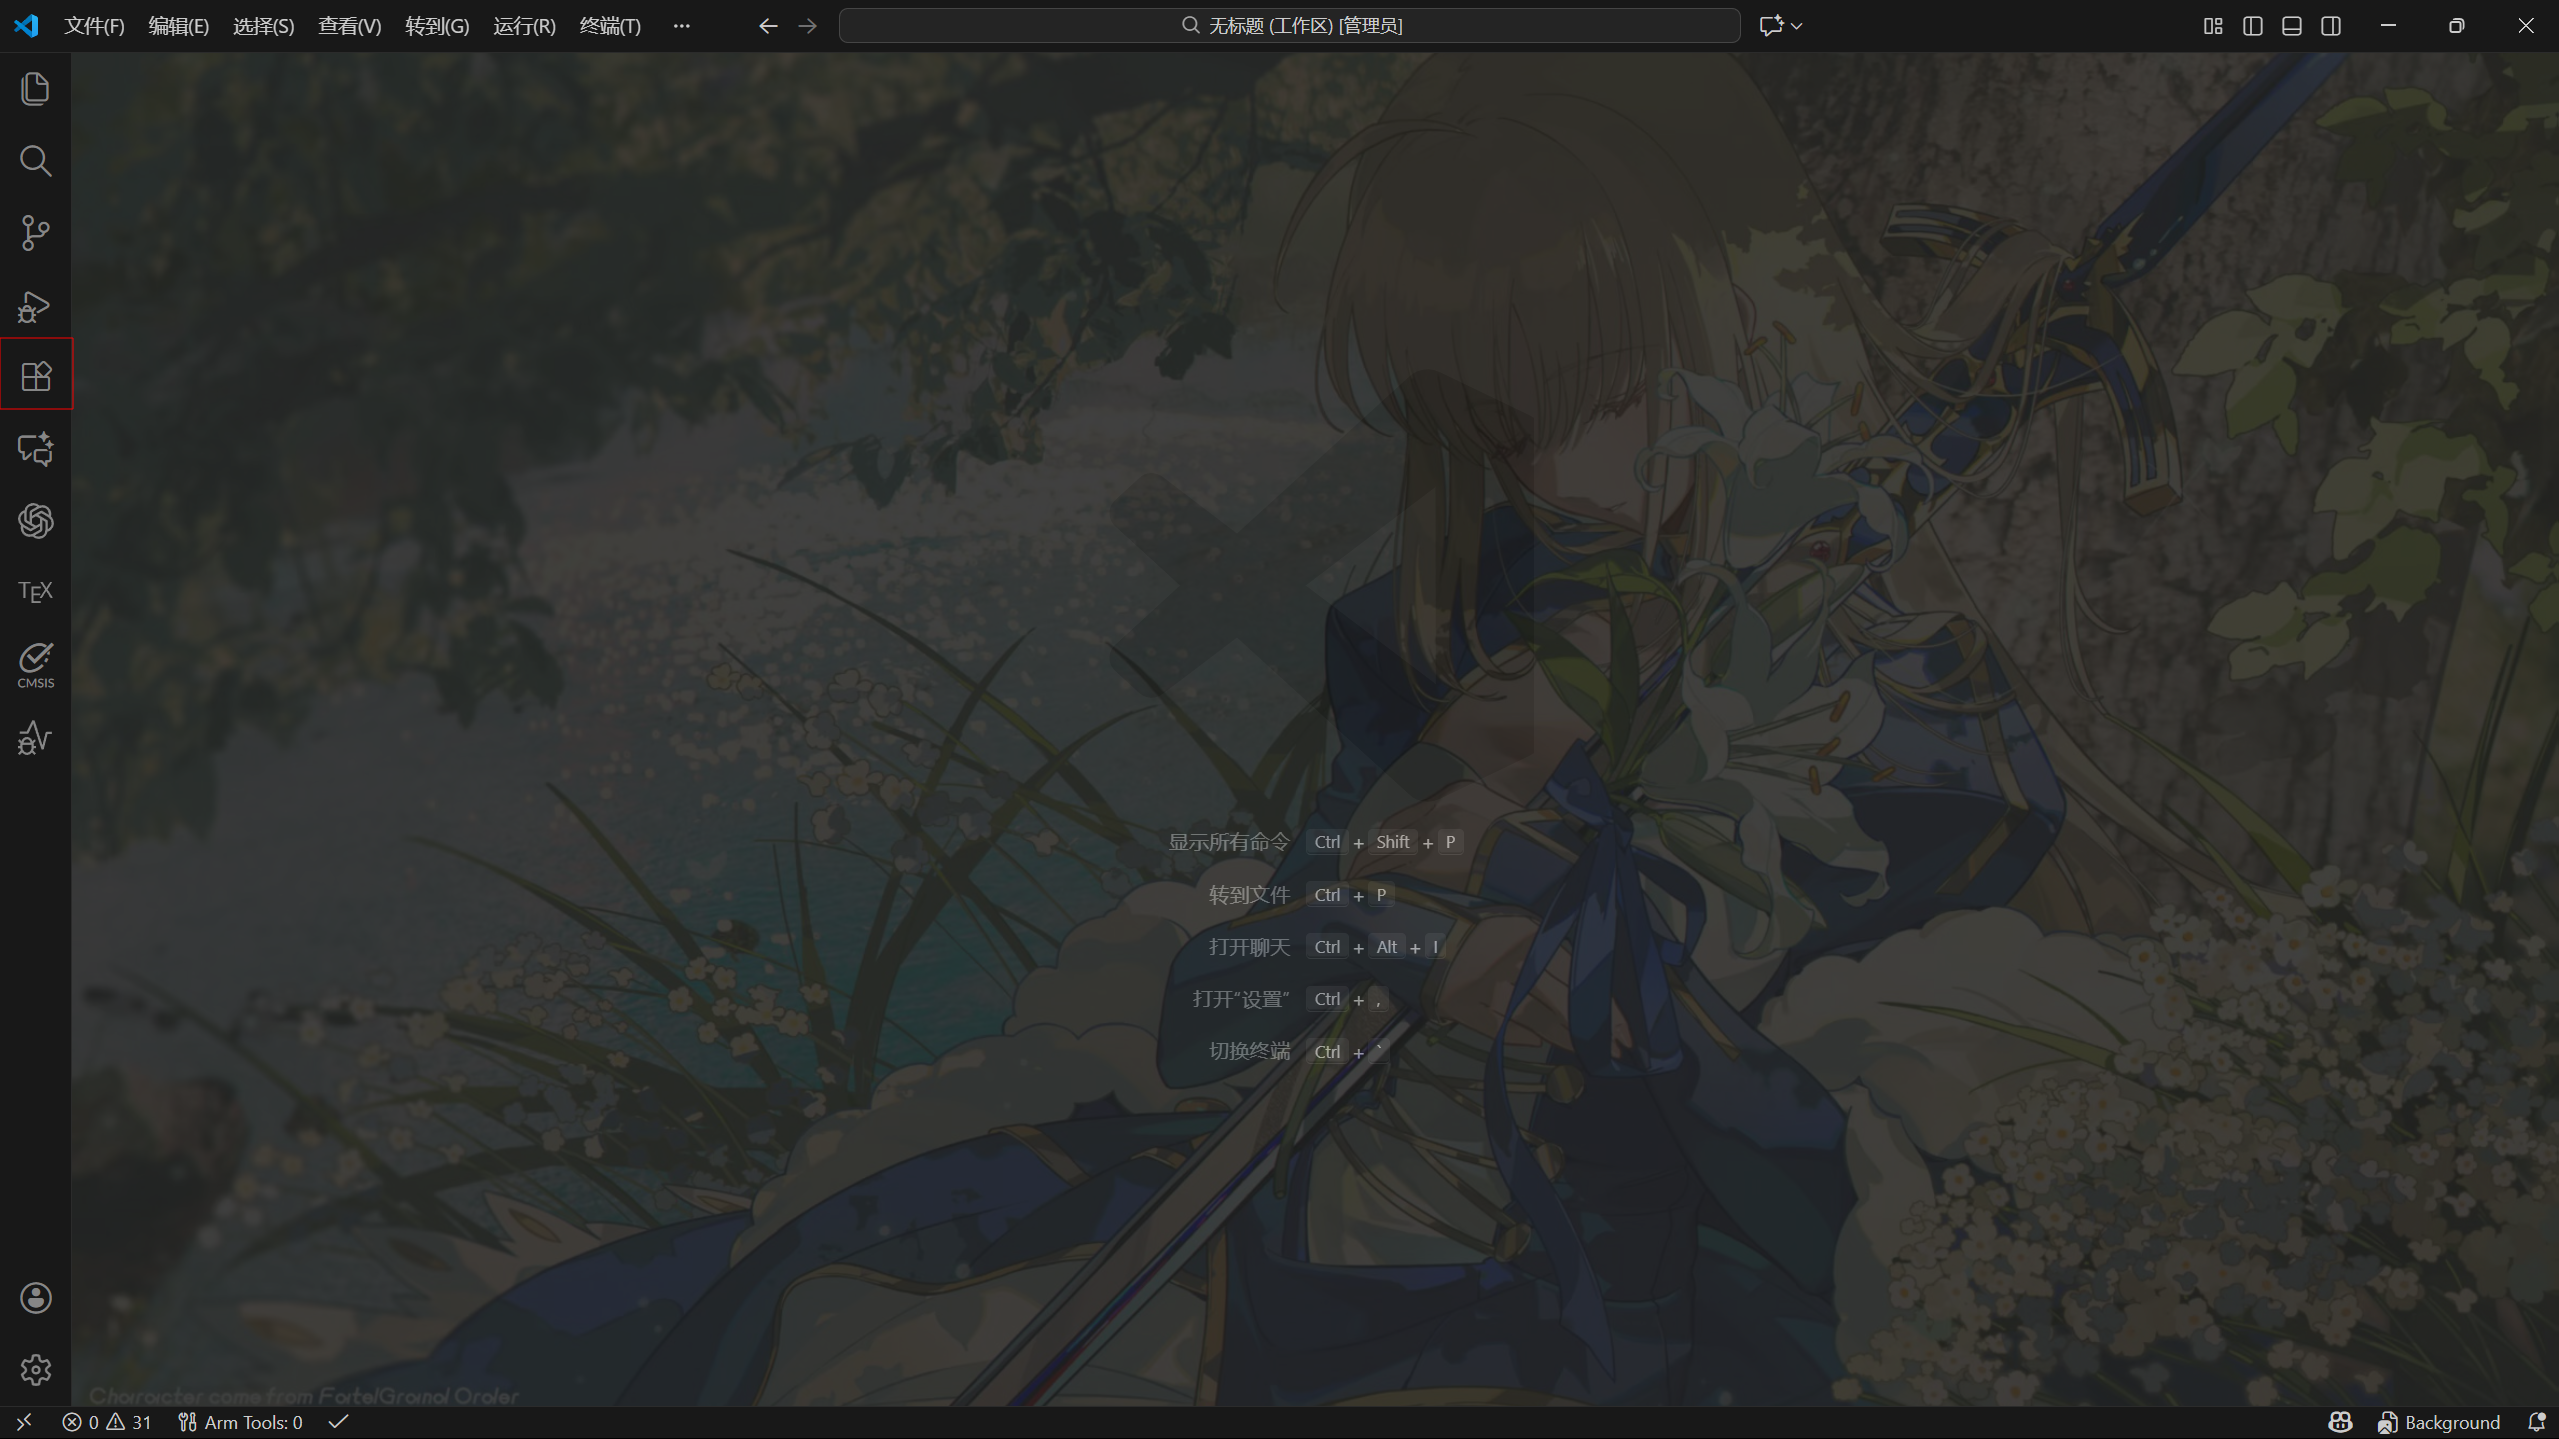
\includegraphics[width=0.8\linewidth]{figures/VScode扩展插件按钮位置.png}
        \caption{VS Code 扩展插件按钮}
    \end{figure}

    \newpage

    \item 在搜索框中输入 \texttt{Python}。
    \item 选择由 Microsoft 发布的 Python 扩展，点击 \textbf{Install} 按钮进行安装。
    \begin{figure}[H]
        \centering
        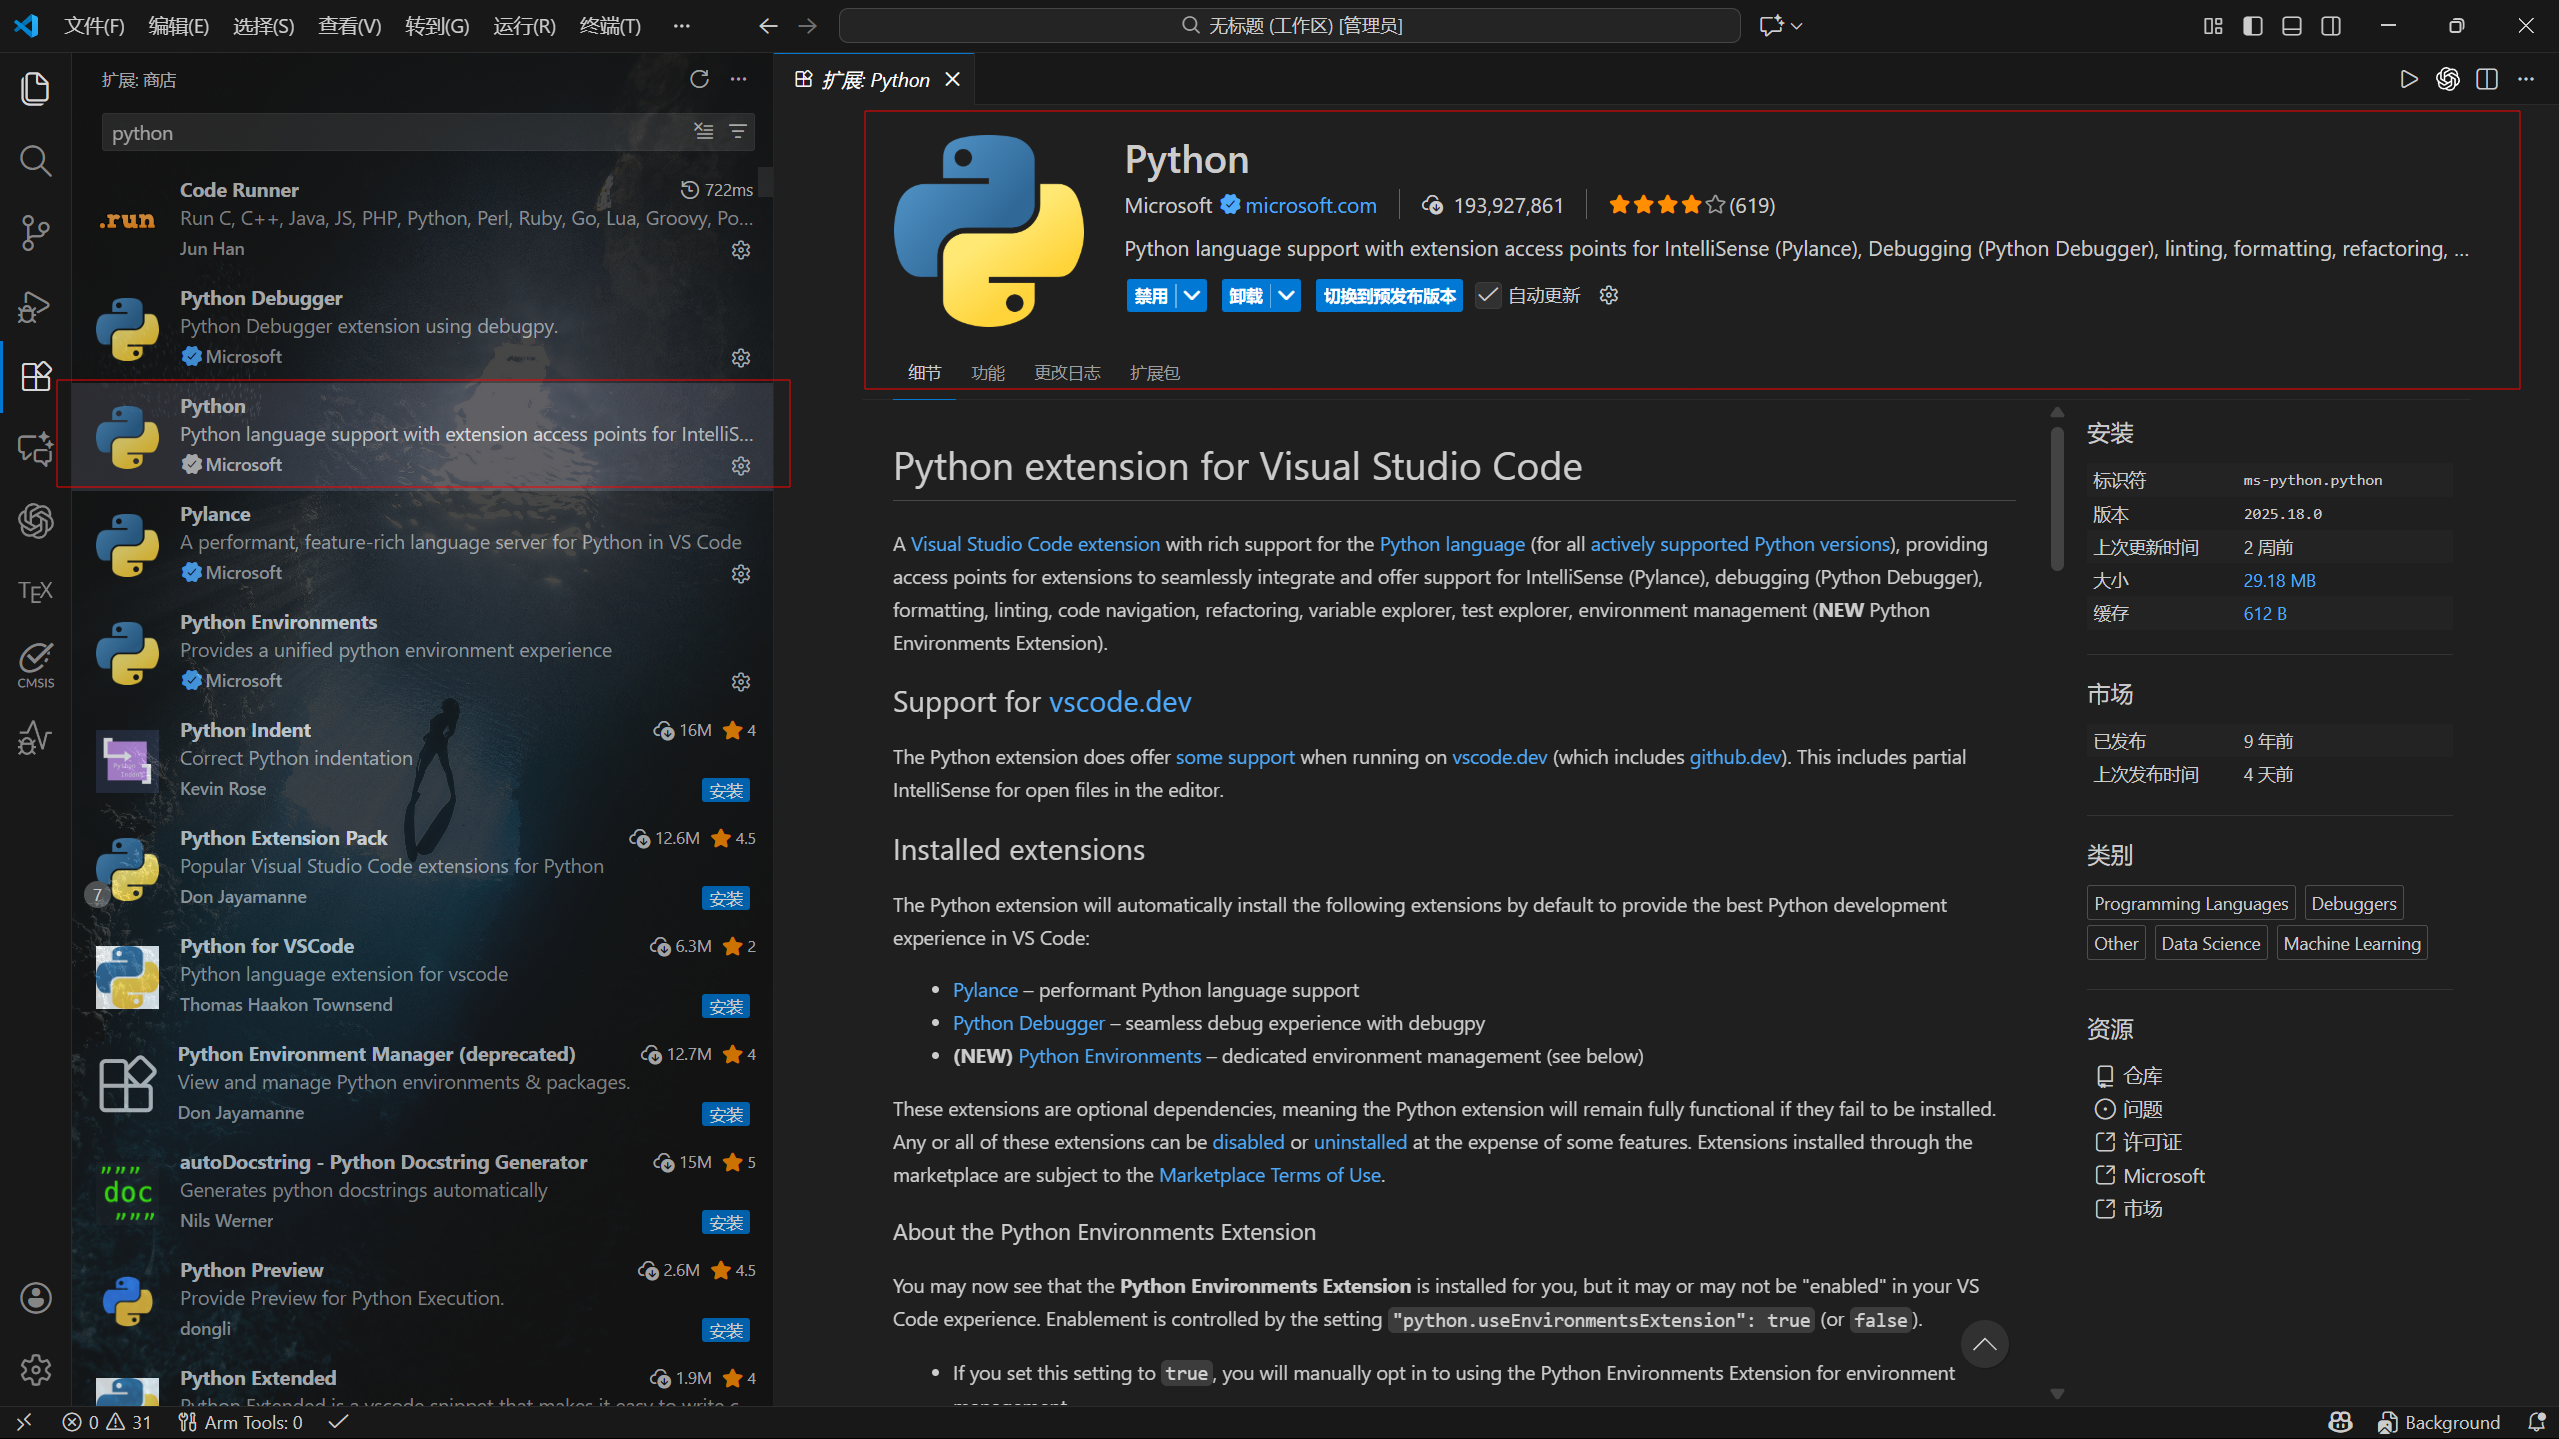
\includegraphics[width=0.8\linewidth]{figures/Python插件.png}
        \caption{安装 Python 插件}
    \end{figure}
\end{enumerate}


\newpage

\subsection{配置解释器作用范围}
安装完插件后，我们需要告诉 VS Code 使用哪个 Python 环境。
\textcolor{red}{按下 \texttt{Ctrl+Shift+P} 打开命令面板，
输入 \texttt{Python: Select Interpreter} 并回车。}

\vspace{1em}
首先我们理顺一点逻辑：在 VS Code 中，
你可以为单个项目（文件夹）配置 Python 解释器，
也可以为整个工作区（Workspace）配置解释器。如果你只选择了一个文件夹，
那么选择的解释器只会对该文件夹生效；如果你选择了多个文件夹组成的整个工作区，那么
选择的解释器会对所有文件夹生效，也就是对整个工作区生效。

也就是说，
你可以选择为某个特定文件夹配置解释器，或者为整个工作区配置一个统一的解释器。
\vspace{2em}


如果你的工作区包含多个文件夹（Multi-root Workspace）
，VS Code 会首先询问你要为哪个文件夹配置解释器，
还是要为整个工作区配置。


\vspace{1em}

比如拿我这里来举例子，我的工作区包含四个文件夹：
\texttt{笔记} 、\texttt{C\_code}、\texttt{Python} 和
\texttt{Lee} 。其中前面两个文件夹主要存放 C 语言代码和笔记，
后面两个文件夹分别存放Python软件和个人项目代码。

所以显而易见，我只希望为 Lee 文件夹单独配置一个 Python 解释器，
而不是为整个工作区配置一个统一的解释器（当然，统一配置也行，因为C语
言项目会自动无视Python环境，两者互不干扰



\begin{figure}[H]
    \centering
    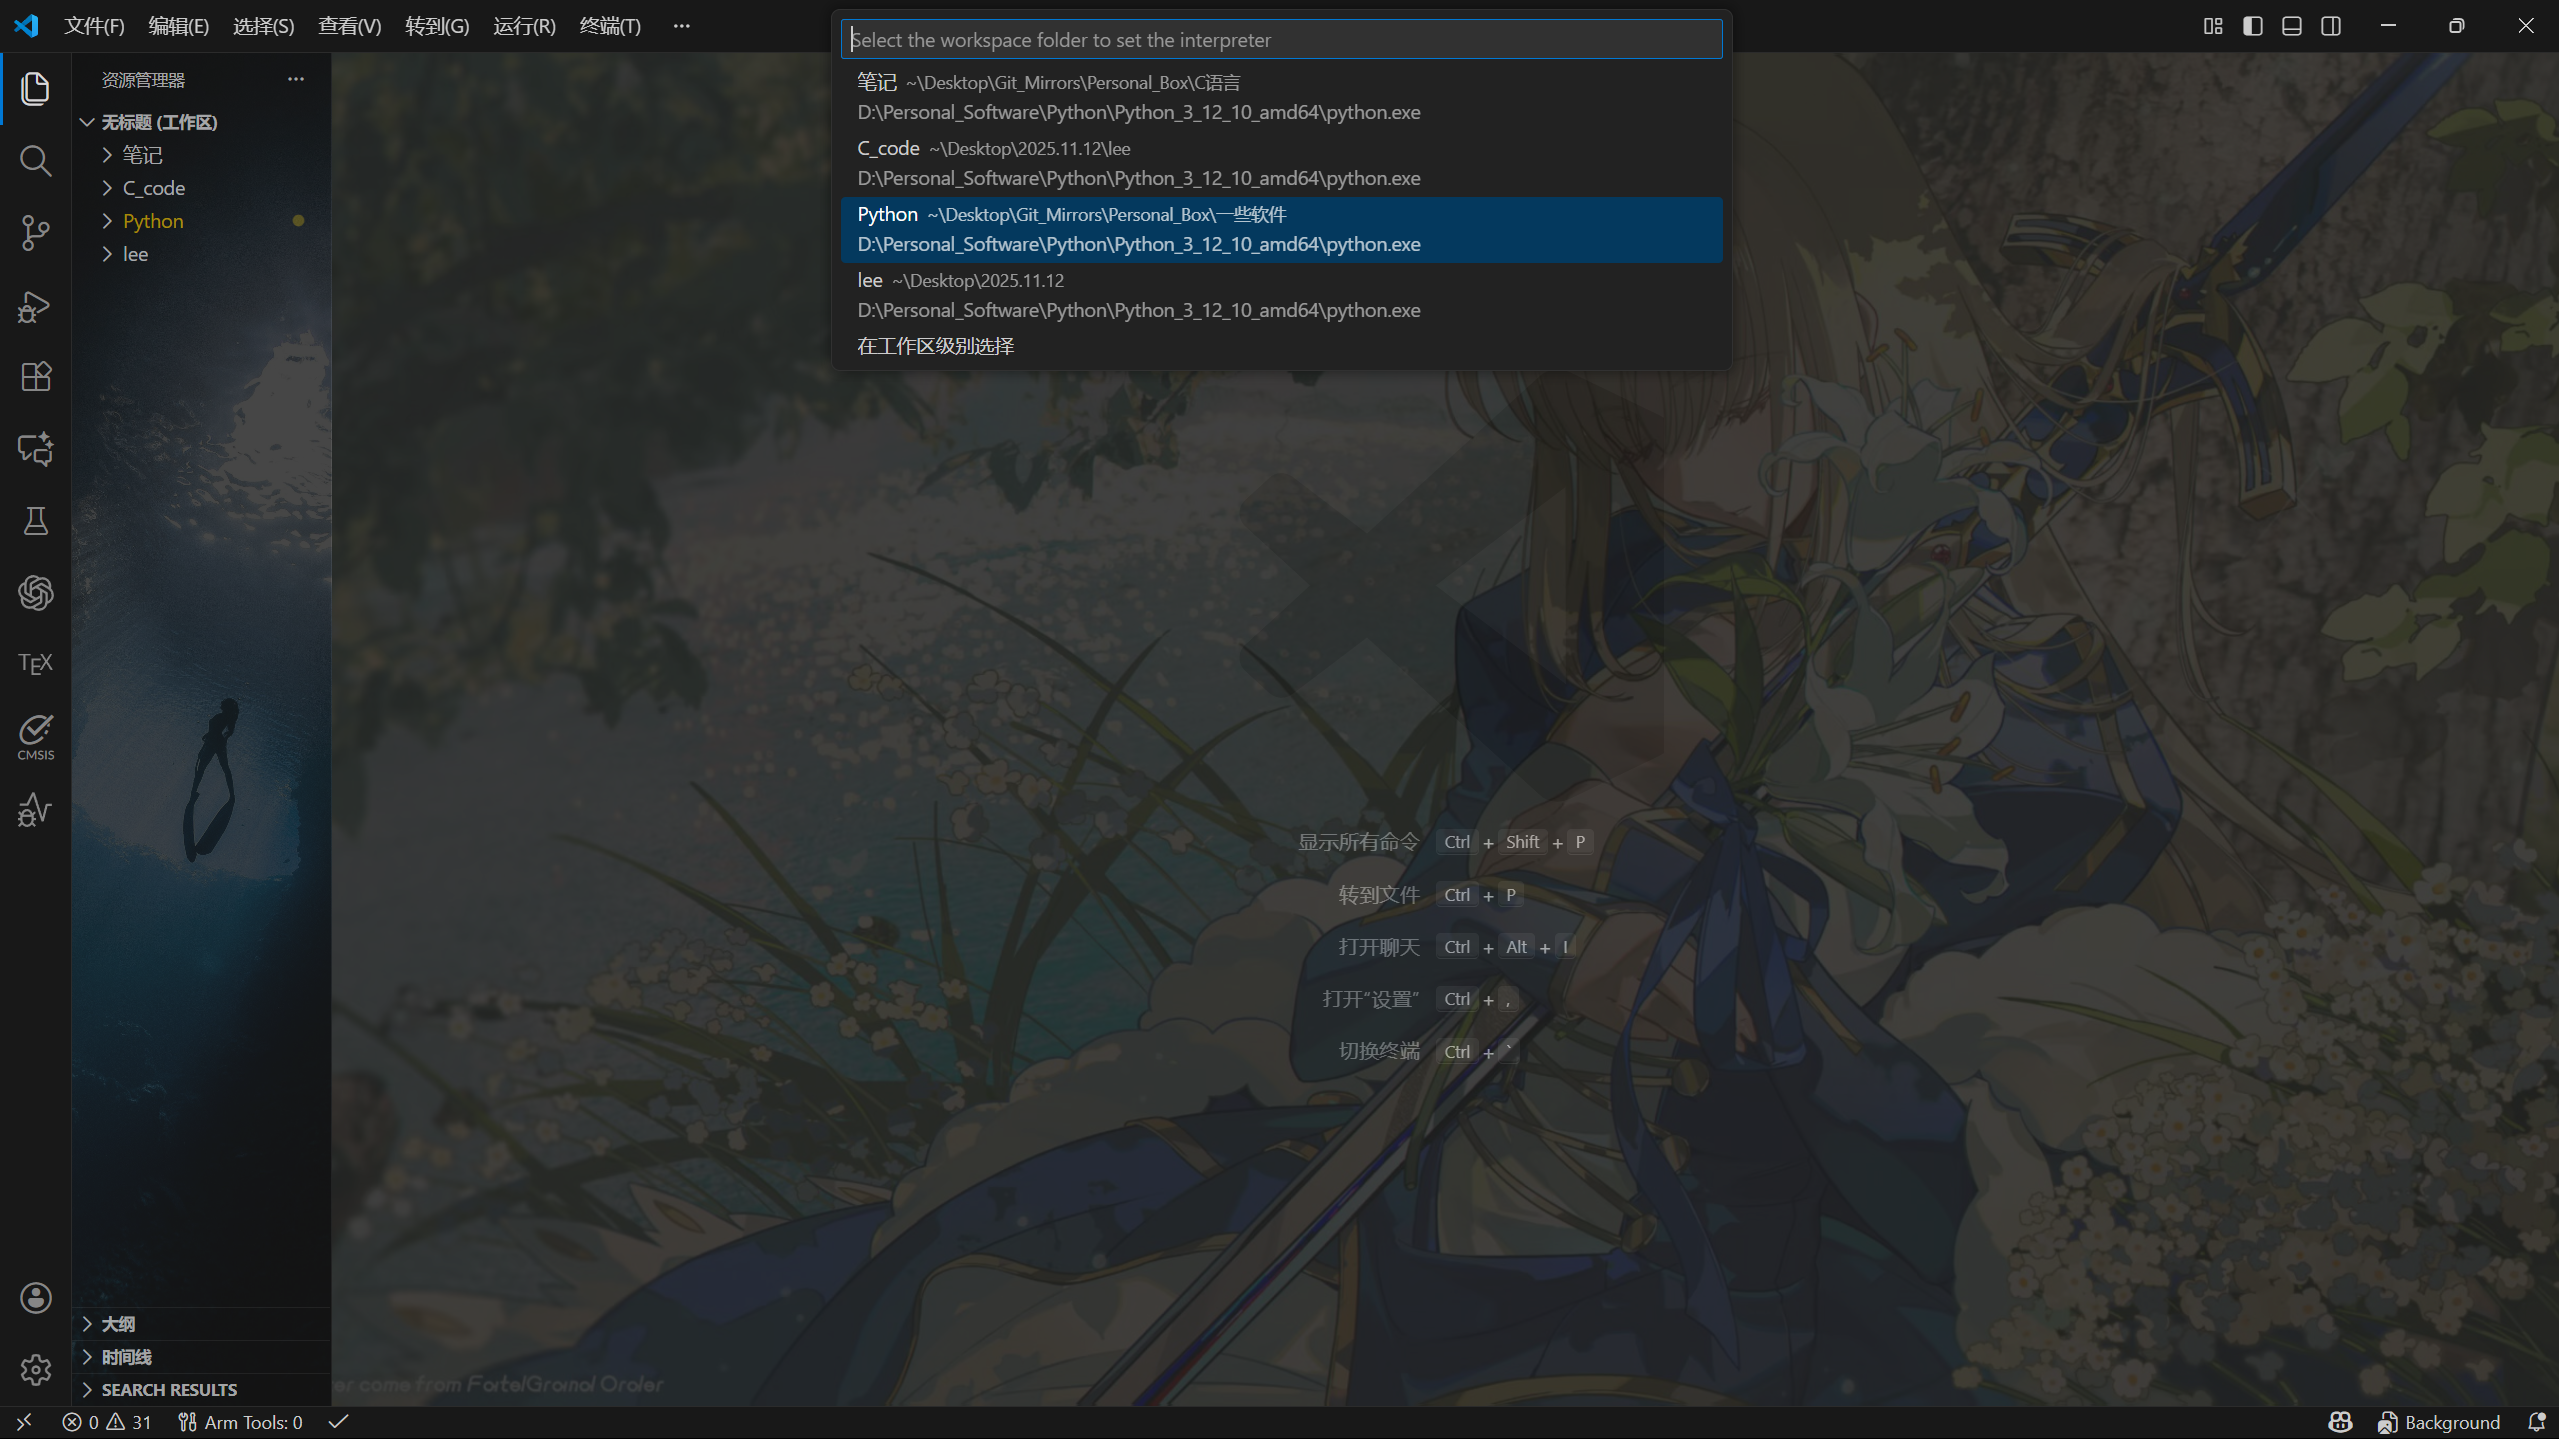
\includegraphics[width=0.8\linewidth]{figures/Python解释器环境选择.png}
    \caption{选择解释器配置范围}
\end{figure}

\textcolor{red}{所以我们鼠标点击想要配置解释器的文件夹名称
（比如 Lee），然后回车确认；如果你想为整个工作区配置，就点击
最下面的\texttt{在工作区级别选择}，然后回车确认。
}

这一步决定了你的解释器设置是仅对特定项目生效，还是对当前打开的所有项目生效。

\newpage

\subsection{选择具体解释器}
确定了配置范围后，VS Code 会弹出一个列表，显示系统中检测到的所有 Python 解释器。


\vspace{2em}

在实际工程中，为了不同的项目开发和团队协作（如果不统一 Python 版本，
团队协作中会发生“代码在你电脑上能跑，在我电脑上直接报错”的尴尬情况），
你的电脑上可能会安装多个 Python 版本（比如 Python 3.8、Python 3.9、Anaconda 等等），
所以这里会列出所有可用的解释器供你选择。

\textcolor{red}{当然对于新手来说，如果你只安装了一个 Python 版本，
那就直接选择它就行了。鼠标点击确认即可
}







\begin{figure}[H]
    \centering
    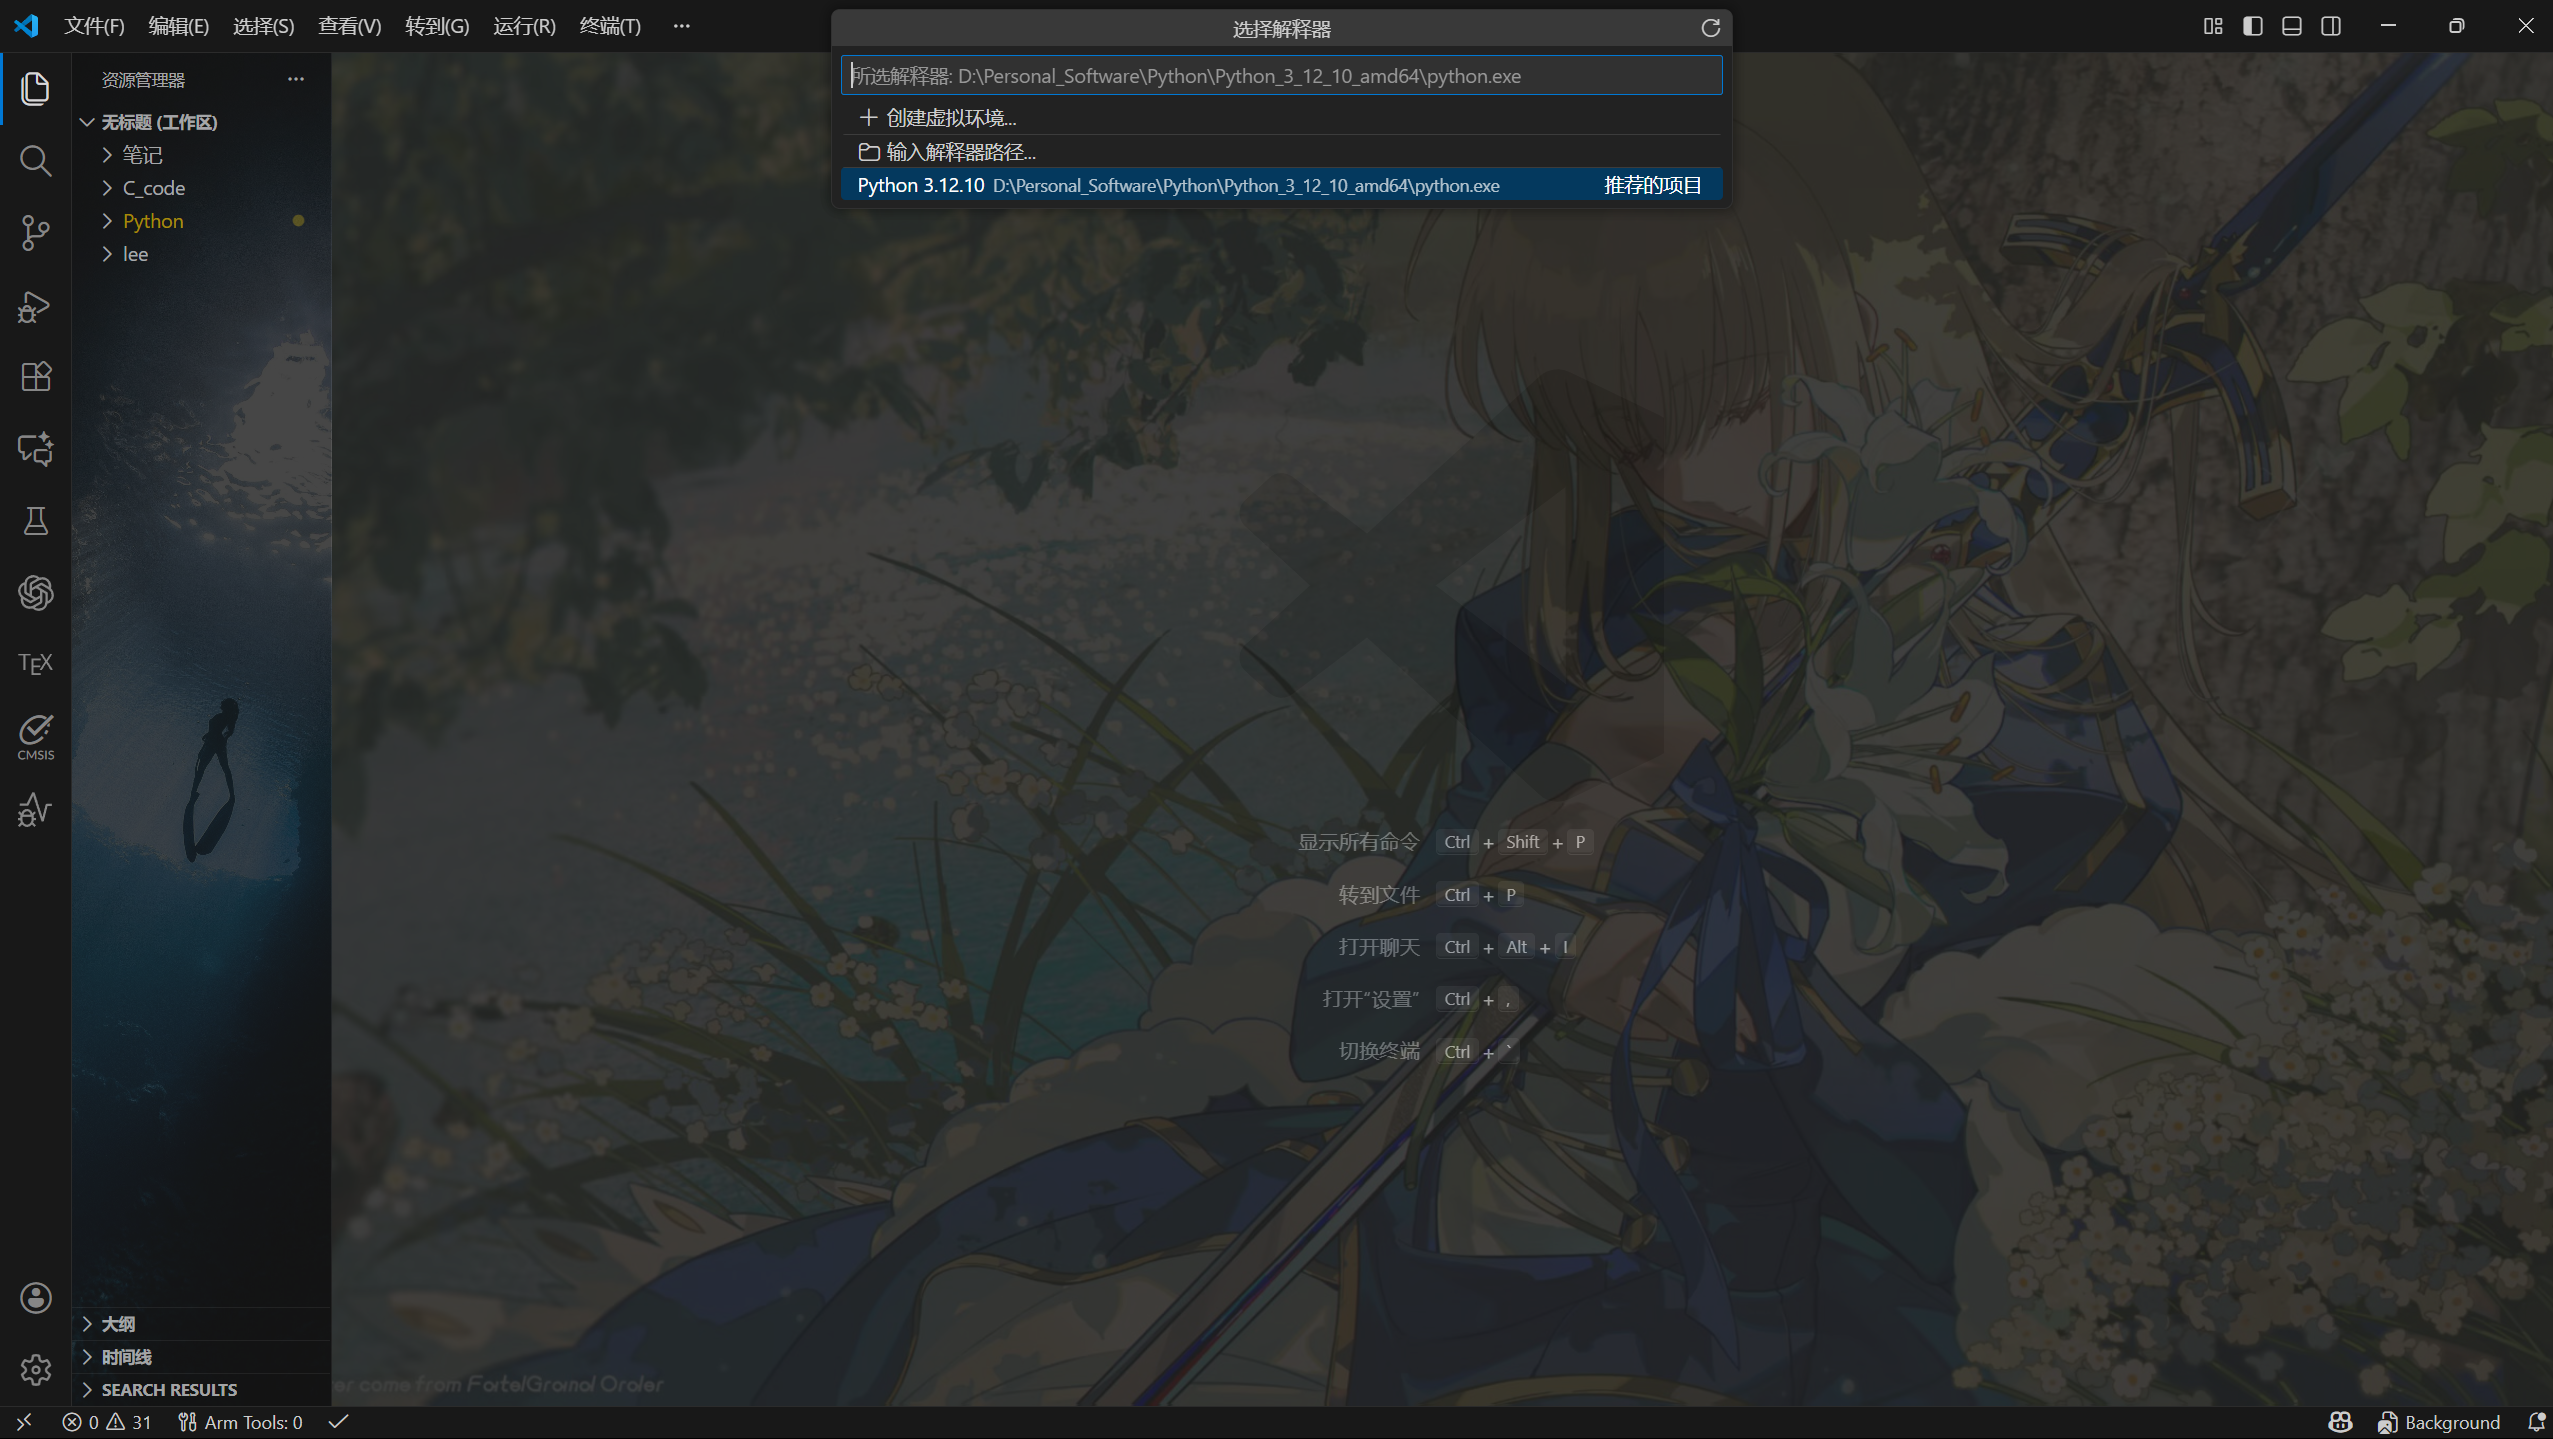
\includegraphics[width=0.8\linewidth]{figures/Python解释器选择.png}
    \caption{选择 Python 解释器}
\end{figure}
在列表中选择你想要使用的 Python 版本（例如 \texttt{Global} 标记的系统 Python，或者 \texttt{Conda} 环境等）。选择后，VS Code 状态栏的右下角会显示当前选中的解释器版本。


\newpage

\subsection{编写 Hello World}
现在环境已经准备就绪，让我们编写第一个程序：
\begin{enumerate}
    \item 在 VS Code 中新建一个文件，保存为 \texttt{hello.py}。
    \item 输入以下代码：
\begin{verbatim}
print("Hello, World!")
\end{verbatim}
    \item 点击右上角的运行按钮（三角形图标），
    或者右键选择 \textbf{Run Python File in Terminal}。

    \textcolor{red}{但我个人更喜欢的运行快捷键是 \texttt{Ctrl+Alt+N}(需要安装 Code Runner 插件)，
    这样可以直接运行当前文件而不调试。}

\end{enumerate}

你将在下方的终端窗口中看到输出：
\begin{lstlisting}{style=python}
Hello, World!
\end{lstlisting}

\newpage 
\subsection{进阶：理解与使用虚拟环境}

对于初学者来说，“虚拟环境”可能是一个比较抽象的概念。但在 Python 开发中，它极其重要。

\subsubsection{为什么需要虚拟环境？}
想象一下，你正在开发两个不同的项目：
\begin{itemize}
    \item \textbf{项目 A}：需要使用 \texttt{Django 2.0} 开发一个老网站。
    \item \textbf{项目 B}：需要使用 \texttt{Django 4.0} 开发一个新网站。
\end{itemize}
Python 的第三方包默认是安装在全局环境中的。如果你在全局环境中安装了 Django 4.0，那么项目 A 可能因为版本不兼容而无法运行；反之亦然。你无法在同一个全局 Python 环境中同时安装两个不同版本的 Django。

\textbf{虚拟环境}就是为了解决这个问题而诞生的。它就像是为每个项目单独准备的一个“工具箱”。项目 A 有自己的工具箱（装有 Django 2.0），项目 B 也有自己的工具箱（装有 Django 4.0）。它们互不干扰。

\subsubsection{虚拟环境会重复安装 Python 吗？}
\textbf{不会。} 这是一个常见的误区。

创建虚拟环境并不是在你的电脑上重新安装一遍 Python 软件。它实际上是创建了一个文件夹（通常命名为 \texttt{.venv} 或 \texttt{venv}），里面包含了一个指向你系统 Python 解释器的“快捷方式”，以及一个独立的 \texttt{lib} 目录用来存放第三方包。

当你激活虚拟环境后，你使用 \texttt{pip install} 安装的任何库，都只会存放在这个项目的 \texttt{.venv} 文件夹里，而不会污染你电脑的全局 Python 环境。

\textcolor{red}{
    \textbf{再次强调：}
    创建虚拟环境\textbf{绝对不是}重复安装 Python 软件！
    它只是在你的项目里建了一个“小房间”，这个房间里有独立的架子用来放包。
    不同的房间（虚拟环境）之间是完全隔离的，
    这样你就可以在房间 A 放 Django 2.0，在房间 B 放 Django 4.0，
    也就是不同的房间用不同的包，而因为房间（虚拟环境）的隔离，不同的
    包不会互相干扰，也不会搞乱你原本干净的系统环境。
}





\subsubsection{如何创建和使用虚拟环境}
\begin{enumerate}
    \item 打开 VS Code 的终端（快捷键 \texttt{Ctrl+\textasciigrave}）。
    \item 确保终端所在的目录是你当前项目的根目录。
    \item 输入以下命令创建虚拟环境：
\begin{verbatim}
python -m venv .venv
\end{verbatim}
    这里的 \texttt{.venv} 是虚拟环境文件夹的名字，你也可以叫别的，但这是约定俗成的习惯。
    \item 创建完成后，VS Code 通常会自动检测到新环境，并右下角弹出提示：“We noticed a new environment has been created. Do you want to select it for the workspace folder?”。点击 \textbf{Yes}。
    \item 如果没有提示，你可以像之前一样，使用 \texttt{Ctrl+Shift+P} -> \texttt{Python: Select Interpreter}，然后在列表中找到带有 \texttt{.venv} 标识的解释器并选择它。
\end{enumerate}

选择后，新建一个终端，你会发现命令行前面多了一个 \texttt{(.venv)} 的标识，这就说明你已经成功进入了虚拟环境。
\newpage
